%PART_3 CHAP_2
\myChapter{R}{ésultats qualitatifs}
%WAIT a Review ok
\begin{resumChap}
Dans ce chapitre, consacré aux résultats qualitatifs, nous présenterons deux éléments indicateurs de l'impact positif du projet dans l'écosystème pour lequel il est destiné.\par%
Nous proposerons donc, dans une première partie, une analyse \tiret{sous forme d'étude de cas} de 10 enseignants ayant participé à la co-conception du Kit robotique pédagogique. Cette analyse présentera comment ils se sont appropriés le kit et comment, de là, ils ont construit leurs propres ressources.\par% 
Puis dans une seconde partie, nous développerons la démarche qui a été mise en place afin de faciliter les processus d'autoformation pour l'enseignant permettant une bonne diffusion du kit. Nous évoquerons également, les structures connexes qui se sont créées: l'association \gui{Poppy Station} et la \textit{start-up} \gui{Pollens Robotics}; pérennisant ainsi le projet dans la durée. De plus, nous rappellerons le rôle des structures préexistantes ayant participé à l'essor du projet. Et enfin nous évoquerons certains des événements périphériques auxquels nous avons participé.
\end{resumChap}{}
\section{Études de cas}\label{sec:entretiens}
    \subsection{Parcours d’appropriation de l'enseignant}
        Il faut prendre en considération que chaque utilisateur, notamment les enseignants, a un spectre de compétences hétérogène. Ainsi leur
        spécialisation dans certains domaines les conduit à exploiter le kit ErgoJr suivant différentes approches. Avant de pouvoir intégrer ses propres processus pédagogiques à la plateforme, l'enseignant doit d'abord la maîtriser, se l'approprier. Dans le cadre de notre kit, il doit apprendre à appréhender la robotique et la programmation.
        Concernant la robotique, que ce soit chez les enseignants déjà conquis par d'autres robots ou chez ceux totalement novices, appréhender la notion de capteur, d'effecteur, de boucle de contrôle ou de monitoring, \etc, ainsi que les spécificités du robot ErgoJr, n'a pas semblé engendrer de difficulté ou susciter de débat particulier durant nos groupes de travail. Cependant, extraire une définition précise de ce qui est ou n'est pas un robot reste périlleux. Mais tous les concepts composant cette définition semblent leur être acquis.
        Concernant la programmation, nous avons observé des comportements distincts dans l'utilisation du langage de programmation visuelle \sht{snap} et de son \sht{api} de contrôle.
        Bien que successeur de langage plus ancien comme \textit{Logo}, la programmation visuelle ne revient que récemment, notamment avec Scratch en 2009; ainsi une majorité des enseignants n'avait jamais manipulé de tels langages. D'un autre coté, certains des enseignants étaient novices en programmation, d'autres manipulaient aisément des langages textuels comme java, C, ou python. Durant leur initiation à \sht{snap} (le langage visuel proposé avec le kit) des distinctions d'usages sont apparues. \par%
        En effet, les enseignants ayant déjà des notions de programmation (textuelle) ont eu une tendance à rechercher les similarités, en terme de fonctionnalité, de fonction, de procédure ou encore de structure, entre \sht{snap} et leur langage textuel préféré. Ainsi, ils adoptaient moins régulièrement la technique d'essais/ erreurs, mais ils y revenaient régulièrement faute de trouver les ponts qu'ils cherchaient. De plus, cette recherche prend un temps non négligeable qui rend l'initiation au langage visuel plus long. À cela, il faut ajouter que certaines notions et fonctionnalités spécifiques à la programmation visuelle leur sont plus longues à acquérir. Cependant, nous avons constaté chez plusieurs enseignants que cette initiation avait profondément changé leur vision de l'informatique et de la programmation; d'après eux, avoir découvert cet autre type de programmation et les spécificités qu'il induit, leur a permis de mieux comprendre et de mieux généraliser des concepts de programmation qu'ils manipulaient quotidiennement en textuel. Pour d'autres enseignants, l'utilisation de tels langages a été complètement éludée au profit de l'usage seul de programmation textuel. Nous voyons donc pour ce profil que l'initiation à la programmation visuelle est plus long et qu'après initiation les enseignants sont rarement réfractaires, que, dans la majorité des cas, ils utiliseront tel ou tel type de programmation suivant leurs besoins (comme avant), et que, rarement, ils modifient drastiquement leur approche en fonction de leurs nouvelles connaissances.\par%
        Concernant les enseignants n'ayant pas, en amont, de connaissance particulière en informatique, nous avons constaté que  l'aspect découverte essai/erreur est très présent. Leur initiation est plus rapide et leur appropriation de ce type de langage meilleure, notamment ils exploitent plus facilement les différentes fonctionnalités spécifiques à \sht{snap}. De plus, ils semblent avoir acquis les bases nécessaires à la construction d'un programme simple (instruction, condition, séquence, boucle, variable, \etc).\par%
        Outre cette distinction dans l'initiation à la programmation visuelle suivant le \textit{background} de l'individu, nous constatons que pour tous, se référer à la documentation n'est pas le première réflexe, ils semblent être d'avantage prompts à consulter des exemples concrets (autre activité présentant les mêmes objectifs ou difficultés) ou à poser une question directement par mail \etou sur le forum. Cependant pour consulter des exemples d'activités déjà réalisées par des élèves, il est nécessaire que l'enseignant ayant fait faire cette activité, partage les résultats de son travail et du travail de sa classe, sans quoi la liste des exemples disponibles restera très succincte. Le partage public de ces contenus a représenté une vraie difficulté, les enseignants trouvant leur travail “pas assez bien”, “trop brouillon”, “pas assez dans les cases du programme officiel”; cependant après de longues discussions, la majorité des contenus nous ont été transmis et sont aujourd'hui disponibles sur le siteweb du projet \href{https://www.poppy-education.org/}{poppy-education.org}~\citeURL{poppy-Education}.
    \subsection{Étude de cas: les enseignants et leurs activités.}
        Durant les phases de conception et d'évaluation, de nombreux acteurs sont venus enrichir notre groupe de travail. Parmi ces acteurs nous retrouvons principalement les membres du projet Poppy Éducation et les enseignants. Parmi eux, une dizaine fait l'objet d'un suivi régulier depuis les prémices du projet. Ainsi nous avons pu observer diverses situations d'enseignement émanant de diverses utilisations du kit, elles-mêmes dépendantes des contraintes environnementales (type de séance: activité / projet, en groupe / en classe entière, \etc; du nombre d'heures et de robots disponibles; \etc) et des connaissances de l'utilisateur (enseignants et élèves). En voici plusieurs exemples:\par%
        D'abord nous pouvons distinguer les enseignants en poste dans des modules de sciences numériques depuis plus d'une décennie et ceux ayant démarré plus récemment.
        %Joël Rivet, enseignant ISN, Lycée Saint Genès, Bordeaux, 15ans exp
        \myPhantom{paragraph}{Joël Rivet, Lycée Saint Genès}
            Ainsi, Joël Rivet, enseignant en ISN au Lycée Saint Genès de Bordeaux, pratique l'informatique avec ses élèves depuis plus de 15ans. Cet enseignant a notamment participé au développement du projet Inorobot (avec le robot Thymio) qu'il continue d'alimenter. Depuis longtemps il exploite différentes plateformes (hardware et software), et crée ses propres contenus et séquences pédagogiques. 
            Un des premiers projets réalisés par ses élèves, cherchait à créer une partie hardware: un labyrinthe; et une partie software de résolution du labyrinthe; s'ajouter une dimension de présentation et de diffusion de leur travail sous forme de vidéo (\cf \href{https://youtu.be/I6sAAKGQ6T4}{Projet labyrinthe}~\citeURL{JR-labyrinthe}).
            Un second projet, s'intéressait aux notions de cinématique directe et inverse (incontournable en robotique) et ceci par la pratique concrète de ces principes mathématiques abstraits avec le robot ErgoJr. Ici aussi le projet se finalisait par une présentation vidéo du travail, le rapport final de l'élève est également disponible sur le forum: \href{https://forum.poppy-project.org/t/presentation-dun-travail-de-cinematique-2d-avec-le-robot-poppy-ergo-jr-1ere-s/2611}{La cinématique 2d avec le robot ErgoJr en 1ere-S}~\citeURL{JR-cinematique-2d}.
            Joël Rivet propose à ses élèves, en début d'année, une liste contenant différentes plateformes et thématiques exploitables dans un projet qu'ils devront réaliser tout au long de l'année; Ce projet se déroule en groupes de 2 à 4. Ainsi de nombreux projets ont été réalisés, dont certains avec l'ErgoJr, d'autres viendront s'y ajouter.\par%
        %Soulard Sylvain, Collège Anatole France, 33410 Cadillac, 15ans exp
        \myPhantom{paragraph}{Soulard Sylvain, Collège Anatole France}
            D'un autre coté, Sylvain Soulard, enseignant au Collège Anatole France de Cadillac, pratiquant également l'informatique depuis plus de 15ans, a opté pour la réalisation d'un projet de plus grande envergure mais commun à l'ensemble des classes: la création d'une reconstitution du \href{https://forum.poppy-project.org/t/activite-ergo-jr-range-des-conteneurs/2505/3}{Reconstitution port automatisé de Rotterdam}~\citeURL{SS-Rotterdam}. Ce projet de classe a été débuté avant l'intégration du kit. Ici l'enseignant a choisi de sélectionner certains éléments du kit afin de l'intégrer dans son projet existant (qui exploitait déjà plusieurs autres plateformes comme le robot Thymio).
            Ici, ces deux enseignants, déjà experts dans la manipulation de ces outils n'ont eu aucun mal à s'approprier et dériver le kit ErgoJr en fonction de leurs besoins techniques et pédagogiques. En revanche, les autres enseignants, ayant moins d'expérience dans la mise en place de telles activités, ont connu une phase d'appropriation plus longue, mais ayant un impact plus important dans leur pratique quotidienne de la discipline.\par%
        %Gilles Lassus, enseignant ICN, Lycée François Mauriac, Bordeaux, now with pollens
        \myPhantom{paragraph}{Gilles Lassus, Lycée François Mauriac}\label{sec:prof-GL}
            Notamment, nous pouvons citer le cas de Gilles Lassus, enseignant en ICN au Lycée François Mauriac de Bordeaux, qui a vu sa vision des sciences du numérique complètement renouvelée avec la découverte de la robotique pédagogique et les ressources associées. Aujourd'hui il travaille (en plus de son professorat) en étroite collaboration avec la start-up Pollens Robotics spin-off du projet Poppy Éducation~\citeS{sec:spineoff}.\par% 
            \begin{figure}[!h]
            \begin{minipage}{0.6\linewidth}
                \centering
                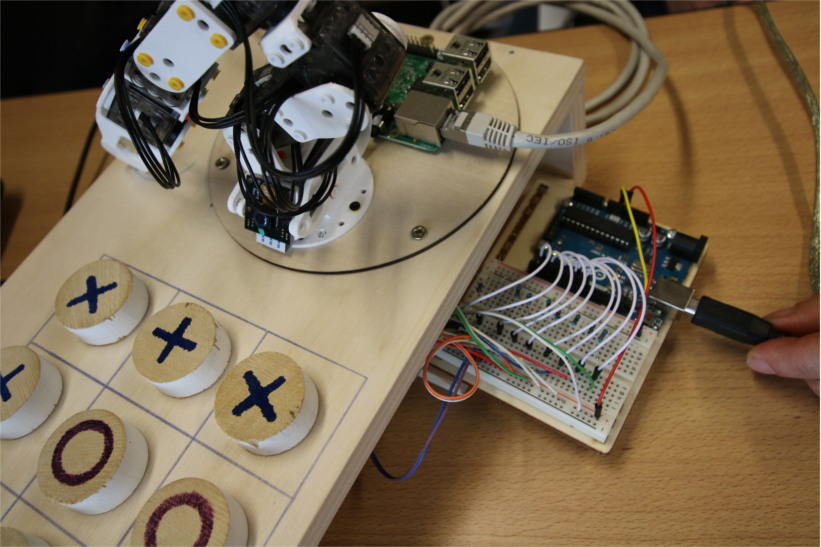
\includegraphics[width=0.9\linewidth]{Figures/GL-tictactoe.jpg}
                \caption[Montage Arduino + Raspberry~Pi sur ErgoJr]{Montage Arduino + Raspberry~Pi\\pour l'activité ErgoJr plays TicTacToe}
                \label{fig:GL-tictactoe}
            \end{minipage}
            \hfill
            \begin{minipage}{0.375\linewidth}
            \myDefautStyle
                Il est d'abord passé par une phase de découverte, exploitant les idées proposées par le groupe de travail (\cf \href{https://www.poppy-education.org/2017/06/06/jouer-a-tictactoe-avec-robot-poppy-ergo-jr/}{ErgoJr - plays - tictactoe}~\citeURL{GL-tictactoe}) puis il a commencé à développer en autonomie ses propres activités (\cf \href{https://forum.poppy-project.org/t/poppyergojr-plays-connect4/2562}{ErgoJr - plays - connect4}~\citeURL{GL-connect4}).
            \end{minipage}
            \end{figure}{}\par%
            Il a ensuite amélioré ses dispositifs en intégrant d'autres éléments (hardware) comme des capteurs photosensibles couplés avec Arduino ou le \textit{LeapMotion}\footnote{ dispositif de reconnaissance de mouvement des mains, pour la réalité virtuelle, créé par Leap Motion, Inc.} (\cf \href{https://forum.poppy-project.org/t/snap-leapmotion-ergo-pierre-feuille-ciseaux/2928}{snap-leapmotion - ErgoJr - plays - pierre, feuille, ciseaux}~\citeURL{GL-LeapMotion}.
            Il intègre également de nouvelles solutions software comme avec sa dernière activité en date via le langage \textit{netsblox} (un dérivé de \sht{snap}) (\cf \href{http://yb-isn.fr/icn2017/blog/2018/01/13/netsblox-envoyer-des-messages-au-pc-da-cote-ou-beaucoup-plus-loin/}{netsblox - Deux ErgoJr à travers le monde}~\citeURL{GL-netsblox}).\par%
        %Youcef Bouchemoua, enseignant ICN, Lycée François Mauriac, Bordeaux, now work with ergo senior
        \myPhantom{paragraph}{Youcef Bouchemoua, Lycée François Mauriac}
            Youcef Bouchemoua, enseignant en ICN au Lycée François Mauriac de Bordeaux a connu une progression assez similaire. Après une phase de découverte avec l'activité chamboule tout, il s'est approprié celle-ci et l'a dérivée en jeu de basket (\cf \href{https://forum.poppy-project.org/t/poppy-ergo-jr-joue-au-basket/3157}{poppy-ergo-jr joue-au-basket}~\citeURL{YB-basket}) où il a intégré ses compétences d'enseignant de physique et mathématiques en ajoutant des séquences sur l'analyse de la trajectoire de la balle en fonction du lancé par le robot. Une activité en parallèle a été réalisée sur le traitement d'image (\cf \href{https://forum.poppy-project.org/t/projet-isn-tri-de-balles-colorees/2511}{projet-isn tri-de-balles-colorees}~\citeURL{YB-triColors}).\par% 
            \begin{figure}[!h]
            \begin{minipage}{0.7\linewidth}
                \centering
                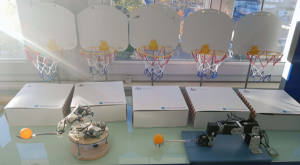
\includegraphics[width=.9\linewidth]{Figures/YB-ErgoJr-ErgoSr.png}
                \subcaption{\label{fig:YB-ErgoJr-ErgoSr}}
            \end{minipage}
            \hfill
            \begin{minipage}{0.29\linewidth}
                \centering
                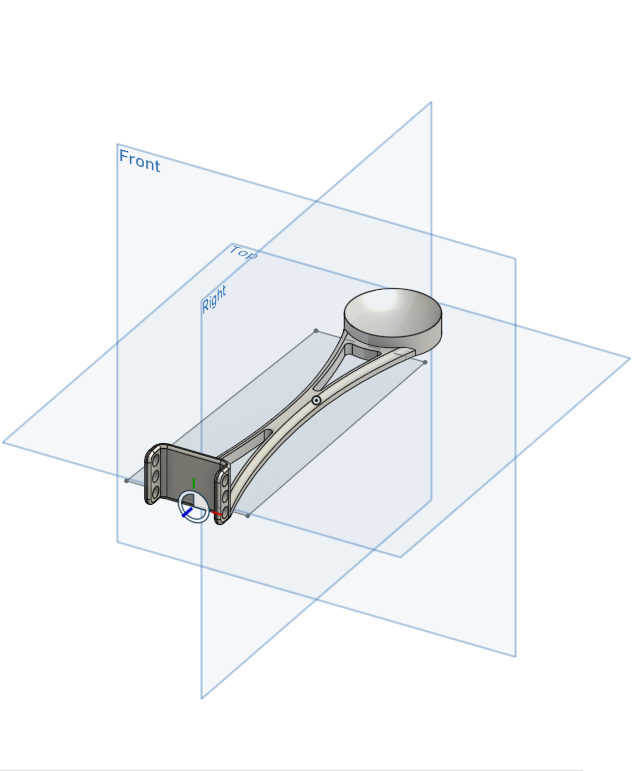
\includegraphics[width=\linewidth]{Figures/TS-ball-luncher.png}
                \subcaption{\label{fig:ball-luncher}}
            \end{minipage}
            \caption[Apprentissage par renforcement avec Ergo Senior]{Apprentissage par renforcement avec Ergo Junior et Senior \& alternative end-effector: The Ball Luncher~\citeURL{TS-luncher}}\label{fig:ErgoJr-ErgoSr-luncher}
            \end{figure}\par%
            L'étape suivante était de réaliser un algorithme d'apprentissage (\cf \href{https://forum.poppy-project.org/t/apprentissage-supervise-avec-poppy-ergo-jr/3427}{apprentissage-supervise avec-poppy-ergo-jr}~\citeURL{YB-learn}). Aujourd'hui, il met en œuvre les algorithmes développés par ses élèves et lui, avec le robot ErgoJr, sur le robot Ergo~Senior (plus onéreux avec ses moteurs \textit{MX-28} mais offrant une précision indispensable à un apprentissage supervisé efficace). Désormais il s'intéresse aux algorithmes développés par l'équipe FLOWERS, et souhaite aller plus loin dans la conception d'activités pédagogiques autour de l'apprentissage automatique et l'IA.\par%
        %Georges Saliba, enseignant ISN, Lycée Victor Louis, Talence, réfractaire snap, absent la 1er anné
        \myPhantom{paragraph}{Georges Saliba, Lycée Victor Louis}
            Un autre exemple concerne, Georges Saliba, enseignant en ISN au Lycée Victor Louis de Talence, qui n'a pas pu suivre les groupes de travail de la première année et qui donc n'a pas effectué la découverte de \sht{snap} et du robot dans le même temps que ses collègues. Il est intéressant de constater que cet enseignant n'est pas adepte des langages de programmation visuelle qu'il juge trop encapsulant, faisant parfois disparaître certains éléments fondamentaux comme le \textit{typage} des variables. Ainsi, il s'est davantage focalisé sur la mise en place d'activités utilisant le langage Python (les seules référencées, en français, à ce jour, sur le site \href{http://www.poppy-education.org}{poppy-education.org} (\cf 
            \href{https://www.poppy-education.org/2016/04/19/tuto-ergojr-python/}{ErgoJr \& Python}~\citeURL{GS-TutoPython}; 
            \href{https://www.poppy-education.org/2016/04/19/tp-ergo-jr-moteurs-et-fonctions/}{TP - ErgoJr - moteurs \& fonctions python}~\citeURL{GS-Python}; 
            \href{https://www.poppy-education.org/2016/04/19/tp-ergo-jr-mouvement-et-lecture-qr-code/}{TP - ErgoJr - mouvement \& lecture de qr-code}~\citeURL{GS-QRcode})\par%
        %Christophe Casseau, enseignant ISN, Lycée Camille Julian, Bordeaux, profils type, utilisation +
        \myPhantom{paragraph}{Christophe Casseau, Lycée Camille Julian}
            Un autre exemple de parcours plus classique mais assez approfondi est donné avec Christophe Casseau, enseignant en ISN au Lycée Camille Julian de Bordeaux qui a mis en place de nombreuses activités avec ses élèves. D'abord avec les quelques exemples à sa disposition au commencement comme avec \href{https://www.poppy-education.org/2017/02/13/ergo-joue-a-tic-tac-toe/}{ergo-joue-a-tic-tac-toe}~\citeURL{CC-tictactoe}. Puis il a très vite mis en scène ses propres activités comme avec l'\href{https://forum.poppy-project.org/t/activite-poppy-ergo-jr-face-au-mur/2809}{activite-poppy-ergo-jr-face-au-mur}~\citeURL{CC-faceAuMur} et laissé ses élèves autonomes dans le développement de leur projet (\href{https://www.poppy-education.org/2017/03/24/poppy-ergo-jr-en-scene/}{poppy-ergo-jr-en-scene}~\citeURL{CC-scene}). Après la création et l'accompagnement sur le plan pédagogique, il s'est ensuite intéressé à la modification du robot en lui-même, notamment en le dotant d'un socle plus stable qu'il partage directement sur le site de son établissement (\href{http://isncaju.wixsite.com/isncaju/single-post/2018/01/18/Impression-socle-Ergo-Jr}{Impression-socle-Ergo-Jr}~\citeURL{CC-socle}).
                \begin{figure}[!h]
                \begin{minipage}{0.315\linewidth}
                    \centering
                    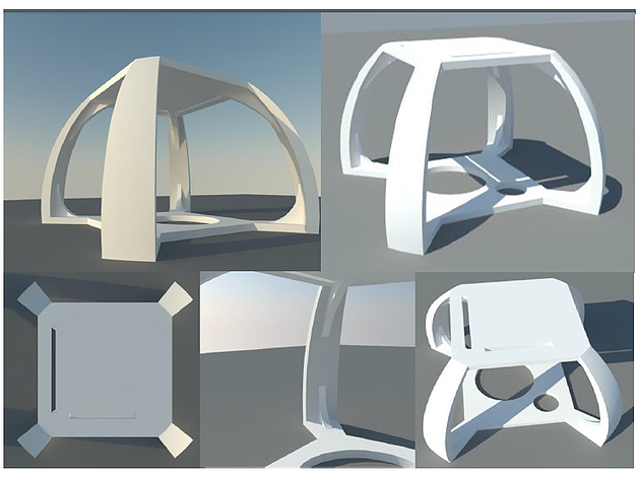
\includegraphics[width=\linewidth]{Figures/CC-socle_num.png}
                    \subcaption{Conception 3D}\label{fig:socle_num}
                \end{minipage}
                \hfill
                \begin{minipage}{0.31\linewidth}
                    \centering
                    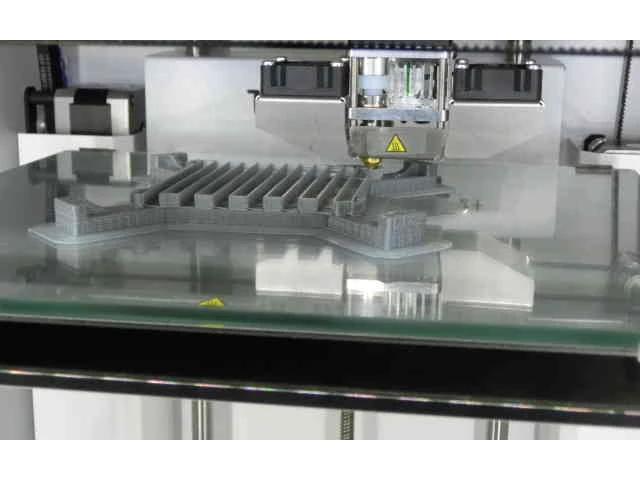
\includegraphics[width=\linewidth]{Figures/CC-socle_print.png}
                    \subcaption{Impression 3D}\label{fig:socle_print}
                \end{minipage}
                \hfill
                \begin{minipage}{0.315\linewidth}
                    \centering
                    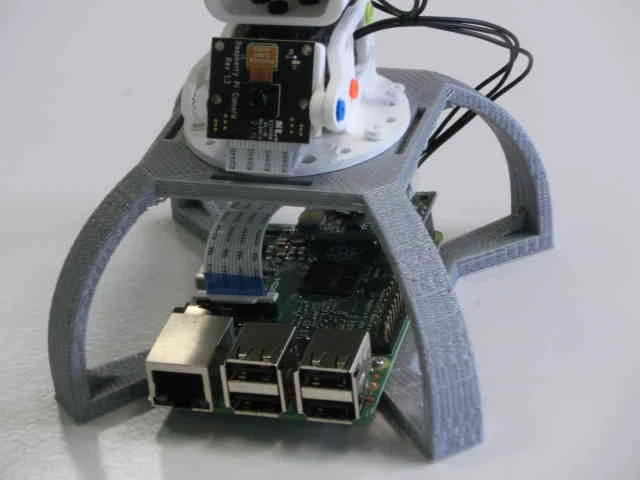
\includegraphics[width=\linewidth]{Figures/CC-socle.png}
                    \subcaption{Résultat}\label{fig:socle_real}
                \end{minipage}
                \caption[Socle alternatif pour ErgoJr]{Socle alternatif pour ErgoJr, réalisation élèves de Mr C Casseau~\citeURL{CC-socle}}\label{fig:socle}
                \end{figure}\par%
            Bien, consciente de l'importance de la diffusion des ressources, il intègre dorénavant cette partie dans le cahier des charges des projets des élèves comme avec ce projet: \href{https://www.poppy-education.org/2017/02/08/ergo-ferme-la-porte/}{ergo-ferme-la-porte}~\citeURL{CC-porte}. Cette enseignant a parfaitement assimilé cet outil dans sa pratique pédagogique.\par%
        %Luc Vincent, enseignant ICN, Lycée des Graves, Gradignan, profils type, utilisation +
        \myPhantom{paragraph}{Luc Vincent, Lycée des Graves}
            Luc Vincent, enseignant en ICN au Lycée des Graves de Gradignan, a lui, bien assimilé cet outil, mais a mis en place moins d'activités avec celui-ci. Il a notamment participé à la mise en place de l'activité \href{https://www.poppy-education.org/2017/03/07/ergo-est-garcon-de-cafe/}{ergo-est-garcon-de-cafe}~\citeURL{LV-cafe} aujourd'hui présent dans le livret pédagogique, et développé le projet \href{https://www.poppy-education.org/2017/12/29/ergo-jr-marin-ohe-ohe/}{ergo-jr-marin-ohe-ohe}~\citeURL{LV-marin} présent sur le site web.\par%
            D'autres enseignants ont eu comme Luc Vincent une expérience avec le kit plus court, comme:
        %Olivier Eloi, enseignant ICN, Lycée Sud Medoc, Le Taillan Médoc.
        \myPhantom{paragraph}{Olivier Eloi, Lycée Sud Medoc}
            Olivier Eloi, enseignant en ICN au Lycée Sud Medoc de Le Taillan Médoc qui a principalement mis en place les activités du livret et soutenu les projets de ses élèves ou 
        %Armelle Grenouilleau, Lycée Jean Moulin, Langon.
        \myPhantom{paragraph}{Armelle Grenouilleau, Lycée Jean Moulin}
            Armelle Grenouilleau du Lycée Jean Moulin de Langon qui s'est limitée à une utilisation plus succinte du kit notamment faute de disponibilité dans ses horaires de cours.\par%
            La disponibilité et l'envie des enseignants pour découvrir, se former, et créer sont primordiales à une bonne appropriation d'un nouvel outil pédagogique. Une fois que celui-ci a bien assimilé les limites et perspectives de cet outil, il est à même de réaliser de nombreux projets. C'est à ce stade, que la disponibilité et l'envie des élèves à découvrir et d'apprendre via cet outil devient primordiale. 
            La robotique baignant actuellement dans l'essor des nouvelles technologies, il est d'apparence assez facile d'obtenir l'envie chez ces élèves de découvrir la plateforme. Mais leur disponibilité va être déterminante dans la réalisation du projet.\par%
        %lycée Kastler, cas particulier STI2D
        \myPhantom{paragraph}{Lycée Kastler}
            Nous pouvons notamment évoquer le cas du lycée Kastler de Bordeaux avec les classes de STI2D, qui a eu une approche différente du fait des programmes et horaire spécifique de cette filière. Par exemple, ils ont mis en place avec Thierry Salem (chef de projet) une compétition avec une restructuration totale de la morphologie du robot ErgoJr pour le rendre mobile: \href{https://forum.poppy-project.org/t/lycee-kastler-projet-ergo-race/2026}{projet-ergo-race}~\citeURL{TS-race}. Plus récemment, c'est Sebastien Prouff enseignant en ICN qui utilise les robots à disposition dans cet établissement. Plus classiquement, il a commencé par utiliser le livret avec ses élèves durant toute l'année (\href{https://forum.poppy-project.org/t/contre-rendu-de-lutilisation-de-poppy-ergo-jr-en-seconde-sicit-base-sur-le-livret-pedagogique-snap-et-ergo-jr/3284}{contre-rendu-de-lutilisation-de-poppy-ergo-jr-en-seconde-sicit}~\citeURL{SP-cr}). Aujourd'hui, il a souhaité aller plus loin notamment en utilisant cet outil comme support technologique pour préparer un dossier pédagogique à partir d'un système issu de l'industrie \etou d'un laboratoire de recherche afin de passer l'agrégation Science Industrielle de l'Ingénieur et ingénierie Informatique. Dans ce dossier il aborde les questions de programmation objet et d'héritage de classe (\href{https://forum.poppy-project.org/t/poppy-heritage-de-classe-python/3778}{pypot heritage-de-classe}~\citeURL{SP-classe}).\par%
            Enfin nous pouvons noter quelques perspectives d'analyses futures avec:
        \myPhantom{paragraph}{Autres exemples}
        %Sebastien Joucla, Yves Laurent 
            Sebastien Joucla \& Yves Laurent du Lycée Grand Lebrun qui ont commencé les activés avec leurs élèves en 2017 et qui ont été formés en 2016. De même avec le Lycée des Métiers la Morlette et ses filières professionnelles (\eg cap coiffure, BAC et BTS Esthétique). Ou encore avec 
        %laurent verdier cf robotcup
            Laurent Verdier du Lycée Saint-Cricq de Pau, et la réussite de ses élèves vainqueurs de la robotcup junior 2018, alors qu'il s'est auto-formé à l'outil, la même année.
    \paragraph{Synthèse}
        Nous voyons donc qu'il existe plusieurs trajectoires dans l'appropriation de ces outils pédagogiques par les enseignants. Parmi cette variété, nous pouvons voir émerger trois types de profils génériques.
        Une fois l'enseignant engagé dans la mise en place d'activités robotiques avec ses élèves, il sélectionne le ou les outils pédagogiques nécessaires à la réalisation des objectifs qu'il s'est fixé.\par%
        Face à un dispositif nouveau, comme avec le kit ErgoJr, l'enseignant doit passer par une phase de découverte des caractéristiques de l'outil lui permettant d'évaluer si les perspectives pédagogiques offertes par l'outil sont bien en adéquation avec ses propres objectifs. Ainsi dans un premier temps, il va manipuler l'outil en suivant les parcours de découverte \textit{clé en main} qu'il réutilisera bien souvent pour une première utilisation en classe. A ce stade, l'enseignant ne crée pas ou peu de contenu, il observe et évalue les réactions de ses élèves face a l'outil pour mieux se l'approprier.\par%
        Ensuite, l'enseignant peut se cantonner à la réutilisation en l'état des contenus diffusés par ses pairs, ou choisir de passer du profil \textit{novice} au profil que nous avons qualifié d'\textit{assimilé}:
        A ce stade, l'enseignant est \textit{à l'aise} avec le kit, il modifie les ressources pédagogiques disponibles pour y injecter ses propres concepts, méthodes et objectifs comme il le fait classiquement dans sa pratique d'enseignement vis-à-vis des autres outils pédagogiques à sa disposition. Cependant, même s'il crée beaucoup de contenu, il préfère les canaux de diffusion traditionnels au partage (public) en ligne comme sur des blogs ou des forums.\par%
        Le troisième profil pourrait être qualifié d'\textit{expert}, car non seulement les enseignants manipulent et transforment les ressources pédagogiques qu'ils trouvent, mais en plus, ils en développent de nouvelles. Il sont à l'aise sur de multiples plateformes, ce qui leur permet, d'une part, de partager facilement leurs ressources en ligne et d'autre part de manipuler et modifier l'outil en lui-même pour l'adapter à leurs besoins, et ceux par l'ajout (ou la suppression) d'éléments software et/ ou hardware sur le kit. Pour acquérir cette expertise les enseignants s'inspirent des différentes ressources qu'ils ont déjà assimilées durant leur carrière via d'autres outils.\par%
        Ces profils sont construits de manière graduelle, sous forme de pallier, cependant nul obligation n'est faite à l'enseignant notamment sur le développement et le partage de ressources. Ainsi, il peut suivant ses disponibilités et affinités rester toute sa carrière  \textit{novice} sur ces questions de robotique en appliquant les ressources fournies, ou en quelques mois devenir un véritable expert du domaine.\par%
        Cependant, ces profils sont génériques et ils peuvent s'appliquer à l'échelle d'un domaine ou d'une plateforme. En effet, dans une certaine mesure, un enseignant est toujours expert de sa discipline puisqu'il l'enseigne. En revanche, à l'échelle d'une plateforme, d'un outil ou d'une technologie spécifique l'enseignant peut être totalement nocive.\par%
        Pour aller plus loin, nous constatons que la première difficulté est d'engager l'individu sur le chemin de l'appropriation  d'une plateforme, notamment si celui-ci n'avait aucune connaissance antérieure sur le domaine d'application de la plateforme. Une fois l'individu engagé, il peut persévérer dans son appropriation de la plateforme et atteindre différents niveaux d'expertise en des temps très variables. Mais, il peut également abandonner la plateforme au profit d'une autre.
        Différentes raisons peuvent motiver cet abandon: une inadéquation entre les attentes sur la plateforme et ses réalités applicatives; une trop grande difficulté de mise en œuvre; un manque de plasticité de la plateforme limitant la création de ressources innovantes.\par%
        Dans notre cas, l'accompagnement réalisé avec les enseignants a limité ce facteur d'abandon. Cependant, dans l'objectif d'une diffusion massive d'un tel kit robotique dans le milieu scolaire et avec la restructuration des programmes officiels (inférant de nouvelles obligations), il est attendu que ce type de comportement émerge. Une difficulté sera alors d'identifier les individus n'ayant pas persévéré dans l'utilisation de la plateforme, puis d'identifier les raisons effectives de cet abandon.
    \subsection{Phase post-conception}
      \paragraph{Un kit \textit{clés en main} pour l'enseignant}
        Comme dit le proverbe \gui{pas de nouvelle, bonne nouvelle}: nous n'avons eu, cette dernière année, que très peu de retours de la part des enseignants suivis. Notamment, la section “support” du forum (servant de relais aux différents bugs et problèmes liés au développement) qui était fortement prisé au début du projet, voit son nombre de nouveaux postes largement diminuer. En revanche, plusieurs indices nous laissent à penser qu'il existe aujourd'hui de nombreux projets mettant en scène le robot Poppy ErgoJr en cours de réalisation. Notamment avec des structures externes~\citeS{sec:externe}.
\section[Disséminer et pérenniser]{Disséminer et pérenniser, le passage à l'échelle}
    \subsection{L'auto-formation}
        \paragraph{Par le faire}
            Essayer de réaliser intuitivement \tiret{par tâtonnement et déduction logique} un objectif est une procédure largement promue dans les domaines du numérique. Les enseignants possèdent un niveau de compétence initiale leur permettant de pouvoir déduire les différentes orientations pédagogiques qu'ils peuvent donner à leur matériel. De plus, ils agissent généralement de façon incrémentale: en rajoutant successivement différents éléments nouveaux aux contenus déjà existants. Ainsi, nous avons pu constater la naissance de nombreux projets (réalisés en autonomie par les enseignants) mettant en jeu différentes ressources et outils additionnels. Ceci leur a permis d'approfondir, d'une part, les connaissances qu'ils avaient sur les plateformes qu'ils manipulaient déjà et, d'autre part, leurs connaissances sur le robot ErgoJr. 
            Mais cette stratégie, n'est pas unique. En effet, les enseignants savent également qu'un problème reste rarement longtemps sans solution. Ainsi, ils savent rechercher et se documenter sur les ressources disponibles (documentation, forum, \etc) pour trouver leurs solutions.
        \paragraph{Sur le web}
            Les ressources sur web, sont de plus en plus fournies. Le site Poppy Éducation en liste une grande partie, d'autres se trouvent également sur le Forum, ou encore sur des blogs et sites web d'établissements scolaires. Dans cette optique d'auto-formation sur le web, un \sht{MOOC} a commencé à être réalisé, cependant il n'a pu être finalisé faute de moyens humains. En revanche, une liste mail de diffusion permet de maintenir le lien entre les utilisateurs ayant une vision pédagogique du robot ErgoJr.
        \paragraph{Par les pairs}
            Sur le terrain, la vie de la communauté Poppy Education est importante, notamment par le contact avec les enseignants et institutions partenaires. %Par ailleurs, son accompagnement dans les usages de manière libre a favorisé sa diffusion: 
            Chaque personne s'est appropriée l'outil en adéquation avec ses propres besoins, sans attentes spécifiques de notre part, et parfois même de manière inattendue. Aujourd'hui, ces personnes diffusent l'outil par leur usage au quotidien (en classe, dans les fablabs, \etc) et, de leur propre initiative, en participant à des évènements (salons, ateliers, formations).  %Par exemple, les enseignants partenaires l'utilisent avec leurs élèves en salle de classe mais aussi lors de formations officielles d'enseignants.
    \subsection{Les structures externes}\label{sec:externe}
        \paragraph{Institutions éducatives}
            En premier lieu, le projet visant à co-créer avec des acteurs de l'Éducation Nationale Française, des partenariats ont été établis avec les institutions éducatives officielles (Rectorat de l’Académie de Bordeaux, Délégation Académique au Numérique Éducatif, établissements scolaires, \etc).
            Ceci a notamment permis de travailler et de co-créer avec des enseignants de l’enseignement d’exploration \sht{ICN} dispensé en classe de Seconde générale de lycée et de l’enseignement de spécialité \sht{ISN} dispensé en classe de Terminale Scientifique. Ainsi différents échanges ont pu avoir lieu avec leurs élèves.
            Comme le montre la figure~\ref{fig:acteurs}, les interactions entre l'équipe Poppy Éducation et ces trois instances (Institutions éducatives officielles, enseignants partenaires et élèves) sont au centre de l'écosystème de création de Poppy Éducation.
        \begin{figure}[!h]
          \centering
          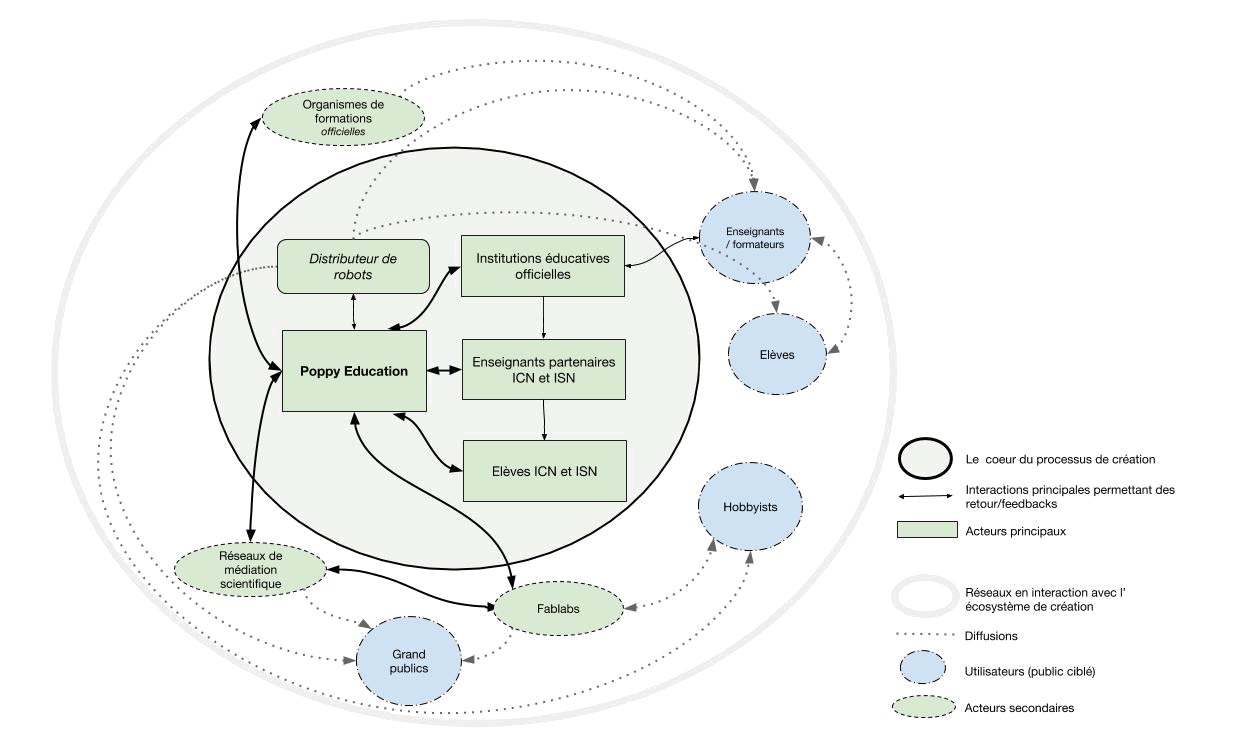
\includegraphics[width=\linewidth]{Figures/Noirpoudre-stakeholders.png}
          \caption{Les acteurs au cœur du processus de création du kit ErgoJr, Noirpoudre~\cite{RI}}\label{fig:acteurs}
        \end{figure}
        \paragraph{Partenariat industriel}
            En second lieu, un partenariat industriel a été mis en place avec le distributeur de robots \cro{Génération Robots} de la région Aquitaine, pour produire et disséminer les kits robotiques que nous développons.
            Ensuite, des collaborations ont été réalisées avec des organismes institutionnels de formation (\cf \bg{ESPE}), Canopé, la Fondation Main à la Pâte, \etc) qui ont pour mission de former les enseignants, notamment aux sciences du numérique.
        \paragraph{Spine off}\label{sec:spineoff}
            Aujourd'hui, deux structures constituent la suite logique du projet Poppy: \Li L'association Poppy Station~\citeURL{station}, qui a pour vocation de promouvoir la robotique open-source dans les domaines de l'éducation et de la formation et \ii la start-up Pollens Robotics qui propose \gui{un service de prestation et formation sur-mesure en robotique et intelligence artificielle pour développer vos propres créatures robotiques}~\citeURL{pollens}
            \begin{figure}[!h]
                \centering\label{fig:spineoff}
                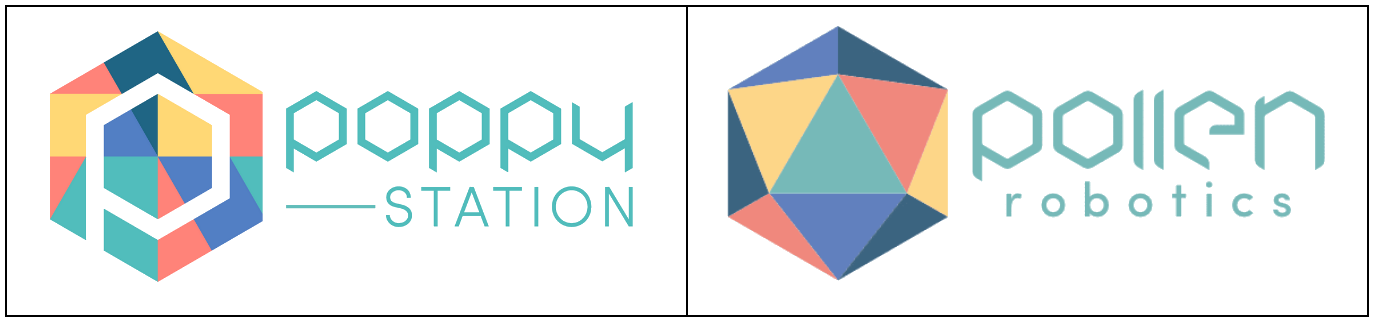
\includegraphics[width=\linewidth]{Figures/Poppy-spineoff.png}
                \caption{Logos, Association Poppy Station et Start Up Pollens Robotics}
            \end{figure}
        \paragraph{Organismes de formation et réseaux de médiation}
            En ce qui concerne les organismes de formation et des réseaux de médiation scientifique, de manière générale leurs demandes étaient traitées au cas par cas. Nous avons privilégié les méthodes pour les rendre autonomes, notamment en leur proposant de suivre une formation adaptée, ce qui a contribué à la diffusion du kit robotique.
            D’autres collaborations ont vu le jour avec des réseaux de médiation scientifique (médiation nationale Inria, Cap'Métiers, Réseau Inmediats, Cap Sciences, \etc) et avec des fablabs qui diffusent les kits robotiques au grand public et aux passionnés.
    \subsection{Les événements connexes}\label{sec:on-stage}\label{sec:canope_danse}
        Le projet Poppy est une communauté open-source basée sur un travail de recherche. Mais cette communauté n'existe pas exclusivement sur le web. De nombreux événements ont permis aux membres de la communauté de se retrouver et de partager leurs projets.
        %\paragraph{Fablab, RobotCup, \etc}
            Un certain nombre d'animations dans des forums et autres colloques ont été réalisées. Ainsi nous avons participé aux \cro{robots makers day}, aux \cro{boussoles du numérique}, à \cro{Connect'thouars}, au \cro{Bordeaux Geek Festival} et à plusieurs formations à l'\sht{ESPE} d'Aquitaine (aujourd'hui nommé \sht{INSPE}). Nous avons également pu participer à d'autres projets mettant en jeu les robots Poppy, comme des cours de danse, des animations dans des médiathèques, des conférences, \etc. C'est durant toutes ces occasions, que nous avons pu mettre en évidence un certain nombre de bugs qui rendaient difficile la mise en place de la plateforme Poppy ErgoJr en l'état. Lors de ces événements, plusieurs activités ont été prototypées. Certaines ont été reprises dans le livret d'activité Poppy ErgoJr, d'autres ont été mises en vidéo, ou exposées sur le forum poppy ou encore le site web. Globalement, cette mise en situation et ces observations ont été particulièrement fructueuses et nous ont permis de dégager plusieurs hypothèses à évaluer et d'imaginer des idées d'activités à créer spécifiques à Poppy ErgoJr.
            %Ainsi, différents réseaux~\citeF{fig:acteurs}, interagissent ensemble pour contribuer à l'amélioration et à la diffusion des kits robotiques.   